\documentclass[10pt]{article}
\usepackage[a4paper,margin=1.8cm]{geometry}
\usepackage[T1]{fontenc}
\usepackage{libertinus}
\usepackage{microtype}
\usepackage{booktabs,tabularx,array,enumitem,tikz,xcolor,fancyhdr,titlesec,caption,multicol,float,needspace}
\usetikzlibrary{arrows.meta,positioning,fit}
\usepackage[colorlinks=true,urlcolor=blue,linkcolor=blue,citecolor=blue]{hyperref}
\definecolor{accent}{HTML}{315C8C}
\definecolor{soft}{HTML}{F1F5F8}
\definecolor{risk}{HTML}{9B2C2C}
\hypersetup{
  pdftitle={Noir Wallet V1 Secure-Element Selection Report},
  pdfauthor={Blockchain Society, IIT Delhi},
  pdfsubject={Secure-element options for Ethereum, Monad, and Solana}
}
\pagestyle{fancy}
\fancyhf{}
\fancyhead[L]{\small Noir Wallet V1}
\fancyhead[R]{\small Secure-Element Selection}
\fancyfoot[C]{\thepage}
\renewcommand{\headrulewidth}{0.4pt}
\setlength{\parindent}{0pt}
\setlength{\parskip}{0.45em}
\setlist[itemize]{leftmargin=1.45em,itemsep=0.15em,topsep=0.2em}
\setlist[enumerate]{leftmargin=1.55em,itemsep=0.2em,topsep=0.2em}
\titleformat{\section}{\Large\bfseries}{\thesection.}{0.45em}{}
\titleformat{\subsection}{\large\bfseries\color{accent}}{\thesubsection}{0.45em}{}
\captionsetup{font=small,labelfont=bf}
\newcommand{\yes}{\textbf{Yes}}
\newcommand{\no}{No}

\begin{document}
\begin{center}
  {\LARGE\bfseries Noir Wallet V1 Secure-Element Selection Report\par}
  \vspace{0.35em}
  {\large Ethereum, Monad, and Solana Compatibility\par}
  \vspace{0.55em}
  {Blockchain Society, IIT Delhi}\\
  \href{https://noirwallet.blocsoc.in}{noirwallet.blocsoc.in}
\end{center}
\vspace{0.5em}
\noindent\rule{\textwidth}{0.6pt}

\textbf{Executive conclusion.}
For V1, use \textbf{NXP EdgeLock SE051C2} with mandatory Platform SCP03 and
replace STM32F401 with a secure-boot/TrustZone-capable MCU. SE051C2 supports
secp256k1 for Ethereum and Monad and, in the correct C2 configuration,
PureEdDSA for Solana; complete Solana support remains conditional on message
encoding, byte-order, and applet-length tests. Microchip TA101 remains fallback. Five compact prototypes
should cost about \textbf{INR 18,600--30,900} when Blockchain Society
does PCB and enclosure design; outsourcing both raises the estimate to about
\textbf{INR 24,900--62,000}. These are September 2026 prototype
estimates, not production quotations.

\section{Short Decision Context}
V0 uses STM32F401CCU6, ATECC608A, SSD1306 OLED, and five buttons. ATECC608A
currently supplies random-command and serial paths; Ethereum keys are derived
on STM32. V1 needs non-exportable wallet keys, a protected local link, verified
boot, rollback resistance, and transaction confirmation bound to the exact
signed payload.

Ethereum and Monad both require secp256k1 ECDSA. Solana requires a separate
Ed25519 key and signing path. SE051C2 can cover all three when exact applet
configuration is verified. Ethereum integration must still normalize low-$s$
signatures and derive recovery parity. Solana must pass exact serialized
message bytes to PureEdDSA rather than a pre-hash; current applet documentation
limits external EdDSA input to 940 bytes in default/AES/EC sessions and 919
bytes in UserID sessions \cite{nxp-apdu}. No secure element supplies correct
transaction parsing or display policy automatically.

\section{Why V0's ATECC Link Is Exposed}
\subsection{\texorpdfstring{I\textsuperscript{2}C}{I2C} transports bytes, not trust}
I\textsuperscript{2}C uses open-drain SDA and SCL lines. Any device physically
connected to those traces can observe bus addresses, command bytes, lengths,
responses, timing, and acknowledgements. Base I\textsuperscript{2}C defines no
peer authentication, confidentiality, message authentication code, or replay
counter. Pull-up resistors provide electrical signaling, not security.

In Noir V0, OLED at \texttt{0x3C} and ATECC608A at \texttt{0x60} share these
lines. A cheap logic analyzer or small interposer can:
\begin{itemize}
  \item reconstruct OLED framebuffer writes and therefore screen contents;
  \item record ATECC opcodes, parameters, serial responses, and random responses;
  \item force low bits, inject/arbitrate traffic, or hold the bus; arbitrary
        bidirectional alteration requires an inline isolating interposer; and
  \item correlate command timing with user actions even when a payload is protected.
\end{itemize}
Current firmware does not establish an encrypted session. Shared-bus topology
also means protecting secure-element commands would not encrypt OLED writes.

\subsection{ATECC608A protection is narrower than a secure channel}
ATECC608A protection is operation-specific, not a persistent secure session:
ECDH/KDF can encrypt selected outputs, while Verify and SecureBoot can MAC
selected responses. It does not protect Random or general traffic and does not
generally authenticate the digest supplied to Sign. Coverage depends on slot
configuration, mode, nonces, TempKey state, and correct host handling.
Unprotected inputs can be substituted or replayed, and all operations remain
deniable by holding/resetting the bus. V0 has not provisioned these mechanisms
\cite{atecc-ds,atecc-io}.

More importantly, ATECC608A signs NIST P-256, not Ethereum/Monad secp256k1 or
Solana Ed25519. Even perfect use of its I/O-protection modes would not turn it
into a non-exportable multi-chain wallet signer. Keeping EVM keys on STM32
leaves key material in ordinary MCU RAM during derivation and signing.

\begin{figure}[H]
\centering
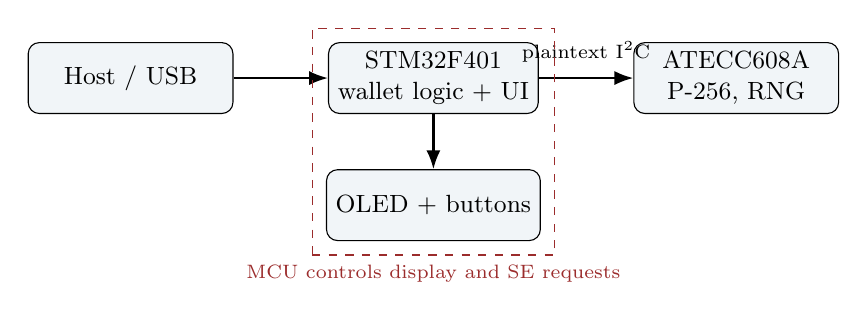
\begin{tikzpicture}[
  font=\small,node distance=0.7cm and 1.2cm,
  box/.style={draw,rounded corners,align=center,minimum width=2.6cm,
              minimum height=0.9cm,fill=soft},
  arr/.style={-{Latex[length=2.4mm]},thick}
]
\node[box] (host) {Host / USB};
\node[box,right=of host] (mcu) {STM32F401\\wallet logic + UI};
\node[box,right=of mcu] (se) {ATECC608A\\P-256, RNG};
\node[box,below=of mcu] (oled) {OLED + buttons};
\draw[arr] (host)--(mcu);
\draw[arr] (mcu)--node[above,yshift=2pt,font=\scriptsize]{plaintext I\textsuperscript{2}C}(se);
\draw[arr] (mcu)--(oled);
\node[draw=risk,dashed,fit=(mcu)(oled),inner sep=5pt,
 label={[text=risk,font=\scriptsize]below:MCU controls display and SE requests}] {};
\end{tikzpicture}
\caption{V0 trust boundary. Stronger secure element does not independently
verify what user saw on MCU-controlled OLED.}
\end{figure}

\Needspace{14\baselineskip}
\section{Candidate Evaluation}
\begin{table}[H]
\centering\scriptsize
\renewcommand{\arraystretch}{1.15}
\begin{tabularx}{\textwidth}{@{}p{2.5cm}c c p{3.1cm}X@{}}
\toprule
\textbf{Device} & \textbf{k1} & \textbf{Ed25519} &
\textbf{Host link} & \textbf{Decision}\\
\midrule
NXP SE051C2 & \yes & \yes &
Platform SCP03; configure \texttt{SCP\_REQUIRED} &
Best fit; verify exact C2 suffix and applet.\\
Microchip TA101 & \yes & \yes &
AES-GCM authorization sessions; SPI/I\textsuperscript{2}C &
Strong fallback; NDA/tooling and provisioning friction.\\
TROPIC01 & \no & \yes &
Forward-secret authenticated SPI &
Open design, but cannot be sole EVM signer.\\
ATECC608A & \no & \no &
Selected I/O-protected operations &
Wrong curves for wallet signing.\\
\bottomrule
\end{tabularx}
\caption{Shortlist. ``k1'' means secp256k1. Configuration and orderable suffix
must be verified before PCB freeze \cite{se051-ds,se051-config,ta101,tropic}.}
\end{table}

\Needspace{10\baselineskip}
\section{How SE051C2 Improves the Link}
\subsection{Mandatory Platform SCP03}
SE051C2 can bind one secure element to its host using three shared AES-128
static keys: Key-ENC, Key-MAC, and Key-DEK. Session establishment mutually
authenticates host and SE using fresh challenges. Key-ENC derives S-ENC;
Key-MAC derives S-MAC/S-RMAC; Key-DEK wraps replacement keys during
\texttt{PUT KEY}. Secure messaging uses AES encryption for APDU data, CMAC for
command and response integrity, MAC chaining, and a per-session command counter.

Noir must set \texttt{SCP\_REQUIRED} with
\texttt{SetPlatformSCPRequest}. In mandatory mode, normal plaintext applet
APDUs are rejected; all subsequent applet APDUs require full command and
response encryption and MAC protection \cite{nxp-binding,nxp-apdu,gp-scp03}.
This blocks passive payload capture, detects modification, authenticates both
ends, and prevents verbatim replay from an old session. It does not stop
real-time relay or malicious requests from an authenticated, compromised MCU.

\subsection{Provisioning rules}
SCP03 only helps when deployed correctly:
\begin{enumerate}
  \item establish first session using development/default keys in a controlled
        environment;
  \item replace default platform KVN 11 with a device-unique customer key set;
        determine whether ordered parts permit customer control of recovery
        KVN 12---generic parts retain an NXP-owned recovery set
        \cite{se051-config};
  \item store host binding material in MCU protected storage. Any HUK-derived
        key needs a documented, domain-separated KDF, key versions, and recovery;
  \item enable mandatory Platform SCP03 and fail closed if setup fails; and
  \item test reset, counter desynchronization, altered MAC, wrong key, downgrade,
        and power-loss recovery before locking production devices.
\end{enumerate}

SCP03 protects SE applet APDUs, not physical addresses/timing, OLED traffic,
USB traffic, transaction parser, or public-chain metadata. A compromised,
authorized MCU can still request a malicious signature. SE051C2 also cannot
verify what OLED displayed. Secure boot and trustworthy confirmation remain
separate controls.

\Needspace{12\baselineskip}
\section{MCU Change and Recommended Architecture}
\subsection{Why STM32F401 should change}
STM32F401 is adequate for V0 bring-up but has no Arm TrustZone-M, immutable
verified-boot service, authenticated debug lifecycle, hardware unique key, or
modern tamper/security partition comparable to newer Cortex-M33 families.
SE051C2 keeps wallet keys non-exportable, but a compromised MCU can still parse
one transaction, display another, and request a signature over attacker data.
Verified boot, secure firmware update, rollback control, protected SCP03 host
keys, and isolated parser/display code therefore belong on the MCU.

\begin{table}[H]
\centering\scriptsize
\renewcommand{\arraystretch}{1.15}
\begin{tabularx}{\textwidth}{@{}p{2.5cm}p{3cm}p{2.7cm}p{2.4cm}X@{}}
\toprule
\textbf{MCU} & \textbf{Security base} & \textbf{Resources / USB} &
\textbf{Prototype price} & \textbf{Assessment}\\
\midrule
STM32U585QII6 & Cortex-M33 TrustZone, RSS secure-install services,
customer-provisioned TF-M/MCUboot OEMiRoT, HUK, active tamper & 160\,MHz,
2\,MB flash, 786\,KB SRAM, USB FS;
7$\times$7\,mm UFBGA & about INR 800--1,100 &
\textbf{Recommended}: strong security, low power, STM32 migration path;
requires professional 0.5\,mm BGA assembly.\\
STM32H573 & Cortex-M33 TrustZone, provisionable ST-iROT, DPA-resistant crypto,
active tamper & 250\,MHz, 2\,MB flash, 640\,KB SRAM, USB FS &
quote required & Strongest ST boot option, but higher cost/power and
unneeded performance. H563 needs customer-protected OEMiRoT.\\
NXP MCXN947 & TrustZone, immutable ROM boot, EdgeLock enclave, PUF, tamper &
dual 150\,MHz M33, 2\,MB flash, 512\,KB SRAM, USB HS/FS &
quote required & Strong non-ST option; secure boot, keys, lifecycle, and
anti-rollback still require provisioning; larger firmware migration and
many unused peripherals.\\
\bottomrule
\end{tabularx}
\caption{Low-quantity India landed estimates. Exact package, stock, GST, and
shipping must be quoted before schematic freeze
\cite{stm32u5,stm32h5,mcxn,mcu-price}.}
\end{table}

STM32U585QII6 is preferred for compact V1 if assembly vendor supports its
132-ball, 0.5\,mm-pitch UFBGA. For hand-assembled early boards, use an
STM32U5 LQFP variant at cost of more PCB area, then migrate package without
changing security architecture.

\subsection{Proposed trust split}
\begin{figure}[H]
\centering
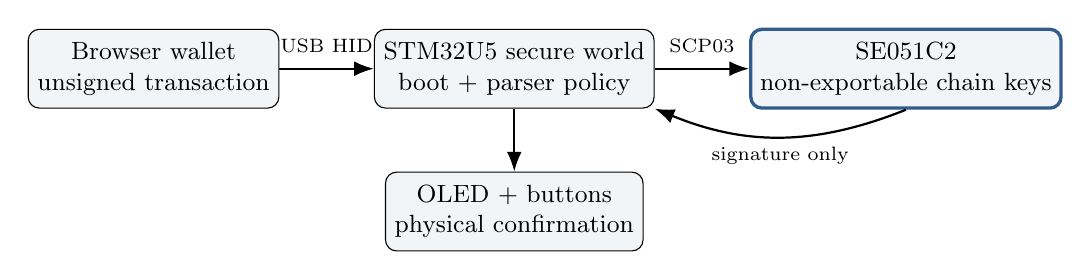
\begin{tikzpicture}[
  font=\small,node distance=0.8cm and 1.2cm,
  box/.style={draw,rounded corners,align=center,minimum width=2.9cm,
              minimum height=1.0cm,fill=soft},
  se/.style={box,very thick,draw=accent},
  arr/.style={-{Latex[length=2.5mm]},thick}
]
\node[box] (host) {Browser wallet\\unsigned transaction};
\node[box,right=of host] (mcu) {STM32U5 secure world\\boot + parser policy};
\node[se,right=of mcu] (se) {SE051C2\\non-exportable chain keys};
\node[box,below=of mcu] (display) {OLED + buttons\\physical confirmation};
\draw[arr] (host)--node[above,yshift=2pt,font=\scriptsize]{USB HID}(mcu);
\draw[arr] (mcu)--node[above,yshift=2pt,font=\scriptsize]{SCP03}(se);
\draw[arr] (mcu)--(display);
\draw[arr,bend left=22] (se.south) to
 node[below,font=\scriptsize]{signature only} (mcu.south east);
\end{tikzpicture}
\caption{V1 trust split. SE051C2 protects wallet keys and APDUs; STM32U5
enforces boot and transaction policy. SE still cannot independently see OLED.}
\end{figure}

\textbf{Control ownership:} SE051C2 owns non-exportable chain keys and SCP03;
STM32U5 owns verified boot, parser, chain policy, and display/button state;
host remains untrusted. Keep OLED off secure-element I\textsuperscript{2}C.
For Ethereum/Monad, sign canonical transaction digest after physical
confirmation. For Solana, pass exact canonical serialized message bytes to
SE051C2 PureEdDSA; do not pre-hash, and reject or explicitly handle messages
over applet input limit.
This reduces key extraction, bus sniffing/modification, replay, and unauthorized
firmware. It does not solve complete-device replacement, denial of service,
host/RPC metadata leakage, or on-chain privacy.

Generate wallet keys inside SE051C2 with minimal sign-only object policies.
Mnemonic recovery that derives/imports keys externally exposes them temporarily
outside SE despite SCP03 transport protection. V1 must define seed backup,
object deletion/replacement, manufacturing authorization, public-key
attestation, and RAM zeroization. Residual threats include MCU/SE fault and
side channels, display/button wiring tampering, validly signed vulnerable
firmware, provisioning-station compromise, APDU relay, and lost binding keys.

\section{Five-Unit Prototype Cost}
\subsection{Assumptions}
Estimate uses India prototype pricing observed in September 2026, 18\% GST
where quoted, one combined component order, a compact four-layer PCB under
100$\times$100\,mm, hand rework or low-volume assembly, and five FDM
enclosures. Foreign listings use a conservative INR 90/USD planning conversion
before GST/shipping. Distributor stock and exchange rates can move component cost
materially. Certification, injection-mould tooling, production provisioning,
test fixtures, and unpaid team engineering time are excluded.
SE051C2 allowance uses low-quantity distributor comparisons rather than
high-volume reel pricing \cite{se-price}.

\begin{table}[H]
\centering\small
\renewcommand{\arraystretch}{1.12}
\begin{tabularx}{\textwidth}{@{}Xr r@{}}
\toprule
\textbf{Five-unit batch item} & \textbf{Low (INR)} & \textbf{High (INR)}\\
\midrule
5$\times$ STM32U5 MCU & 4,000 & 5,500\\
5$\times$ SE051C2 secure element & 2,250 & 3,500\\
5$\times$ SSD1306 OLED module/panel & 500 & 1,150\\
Buttons and user-interface parts & 150 & 400\\
USB-C, ESD, power, clocks, passives, connectors & 1,250 & 2,350\\
Five four-layer PCBs & 2,500 & 2,500\\
Stencil & 1,500 & 1,500\\
Assembly, BGA placement, and rework & 1,500 & 4,000\\
Five FDM-printed enclosures & 1,500 & 4,000\\
Shipping, solder, headers, and consumables & 1,000 & 2,000\\
\midrule
\textbf{Recurring batch subtotal} & \textbf{16,150} & \textbf{26,900}\\
15\% prototype contingency & 2,423 & 4,035\\
\textbf{Team-designed batch total} & \textbf{18,573} & \textbf{30,935}\\
\textbf{Effective cost per unit} & \textbf{3,715} & \textbf{6,187}\\
\bottomrule
\end{tabularx}
\caption{Cash estimate for five functional prototypes built together.}
\end{table}

\subsection{Design-cost scenarios}
Existing V0 CAD and firmware reduce work, but V1 needs a new schematic, PCB
layout, and enclosure around the final board. If Blockchain Society performs
this work, cash NRE is near zero but engineering time is not free. Indian
service listings put schematic plus PCB layout around INR 3,000--12,000 and
basic-to-medium enclosure CAD around INR 2,500--15,000
\cite{pcb-design-cost,pcb-design-upper,cad-cost}. Adding these to recurring subtotal and applying
15\% contingency gives an \textbf{outsourced total of roughly INR
24,900--62,000}, or \textbf{INR 4,980--12,400 per unit} across five.

PCB fabrication references list five two-layer boards at INR 1,500 and five
four-layer boards at INR 2,500 including GST/delivery; a metal stencil is
INR 1,500 \cite{pcb-fab-cost}. OLED listings range from INR 99 to INR 229
including GST \cite{oled-cost}. FDM service estimates vary by weight, time,
material, finish, and minimum order; INR 300--800 per compact enclosure is a
planning allowance, not a quote \cite{print-cost}.

\section{Prototype Gates and Final Decision}
\begin{enumerate}
  \item Confirm exact SE051C2 suffix supports secp256k1, Ed25519, and Platform
        SCP03, then configure \texttt{SCP\_REQUIRED}; do not
        route PCB from family-name assumptions.
  \item Bring up STM32U5 verified boot, rollback protection, debug lifecycle,
        TrustZone partition, and protected host binding keys.
  \item Verify Ethereum low-$s$/recovery parity, Monad chain-ID policy, and
        Solana Ed25519 vectors against independent software.
  \item Capture I\textsuperscript{2}C before and after SCP03; require encrypted,
        MACed APDUs and rejection of plaintext fallback.
  \item Test wrong keys, replay, altered MAC, reset, downgrade, power loss,
        screen/signed-payload mismatch, and seed zeroization before locking devices.
\end{enumerate}

\textbf{Decision:} prototype SE051C2 with STM32U585. Keep TA101 as procurement
fallback. Do not use TROPIC01 as sole signer until it supports documented
secp256k1 signing. Separate secp256k1 and Ed25519 objects and chain policies.

\clearpage
\footnotesize
\begin{multicols}{2}
\begin{thebibliography}{99}
\setlength{\itemsep}{0pt}
\setlength{\parskip}{0pt}
\bibitem{se051-ds}
NXP, \href{https://www.nxp.com/docs/en/data-sheet/SE051.pdf}
{SE051 Data Sheet}.
\bibitem{se051-config}
NXP, \href{https://www.nxp.com/docs/en/application-note/AN12973.pdf}
{AN12973: SE051 Configurations}.
\bibitem{atecc-ds}
Microchip, \href{https://ww1.microchip.com/downloads/aemDocuments/documents/SCBU/ProductDocuments/DataSheets/ATECC608A-CryptoAuthentication-Device-Summary-Data-Sheet-DS40001977B.pdf}
{ATECC608A Summary Data Sheet}.
\bibitem{atecc-io}
Microchip, \href{https://ww1.microchip.com/downloads/en/Appnotes/00002589A.pdf}
{AN2589: Differences Between the ATECC608A and ATECC508A
CryptoAuthentication Devices}.
\bibitem{nxp-binding}
NXP, \href{https://www.nxp.com/docs/en/application-note/AN12662.pdf}
{AN12662: Binding a Host Device to EdgeLock SE05x}.
\bibitem{nxp-apdu}
NXP, \href{https://community.nxp.com/pwmxy87654/attachments/pwmxy87654/secure-authentication/1762/1/AN12543.pdf}
{AN12543: SE05x IoT Applet APDU Specification}.
\bibitem{gp-scp03}
GlobalPlatform, \href{https://globalplatform.org/wp-content/uploads/2019/12/GPC_2.3_D_SCP03_v1.1.2.6.pdf}
{Secure Channel Protocol '03'}.
\bibitem{ta101}
Microchip, \href{https://ww1.microchip.com/downloads/aemDocuments/documents/SCBU/ProductDocuments/DataSheets/TA101-CryptoAutomotive-Summary-Data-Sheet-DS40002529.pdf}
{TA101 Summary Data Sheet}.
\bibitem{tropic}
Tropic Square, \href{https://www.tropicsquare.com/tropic01}{TROPIC01}.
\bibitem{stm32u5}
STMicroelectronics, \href{https://www.st.com/resource/en/datasheet/stm32u585ai.pdf}
{STM32U585 Data Sheet}.
\bibitem{stm32h5}
STMicroelectronics, \href{https://www.st.com/resource/en/datasheet/stm32h573ai.pdf}
{STM32H573 Data Sheet}.
\bibitem{mcxn}
NXP, \href{https://docs.nxp.com/bundle/MCXNP184M150F70/page/topics/front_matter_content_1.html}
{MCXN947 Product Data}.
\bibitem{mcu-price}
DiGi-Electronics, \href{https://www.digi-electronics.my/my/products/detail/stmicroelectronics/STM32U585QII6/11152597.html}
{STM32U585QII6 Unit Price Listing}, accessed September 2026.
\bibitem{se-price}
Octopart, \href{https://octopart.com/part/nxp-semiconductors/SE051C2HQ1%2FZ01XDZ}
{SE051C2 Distributor Comparison}, accessed September 2026.
\bibitem{pcb-design-cost}
RoboThings, \href{https://robothings.in/pcb-design-prototyping-services/}
{PCB Design and Prototyping Services}, accessed September 2026.
\bibitem{pcb-design-upper}
HBeonLabs, \href{https://www.hbeonlabs.in/pcb-design-service-10313366.html}
{PCB Design Service}, accessed September 2026.
\bibitem{cad-cost}
RoboThings, \href{https://robothings.in/product-casing-enclosure-design-service/}
{Product Casing and Enclosure Design Service}, accessed September 2026.
\bibitem{pcb-fab-cost}
WHYPCB, \href{https://www.whypcb.com/pcb-prototype-service-india}
{India Prototype PCB Pricing}, accessed September 2026.
\bibitem{oled-cost}
Robu, \href{https://robu.in/product/0-96-inch-oled/}
{SSD1306 128$\times$64 OLED Listing}, accessed September 2026.
\bibitem{print-cost}
Zbotic, \href{https://zbotic.in/3d-printing-costs-india-calculate-material-and-electricity/}
{India 3D-Printing Cost Guide}, accessed September 2026.
\end{thebibliography}
\end{multicols}
\end{document}
